\chapter{Resultados}
\label{cap:resultados}
En este capítulo se describen los resultados obtenidos al aplicar el método de trabajo presentado en el capítulo \ref{cap:metodologia} usando la metodología \gls{pud}.

\section{Requisitos del sistema}
A continuación se muestran los requisitos funcionales y no funcionales del sistema junto a una breve descripción.

\subsection{Requisitos funcionales}
Se han dividido los requisitos funcionales según la clasificación descrita en la sección \ref{sub:obtencionrequisitos}. Cabe notar que en este documento se refiere como usuario al docente que utiliza la aplicación.

Requisitos \textit{Must have}:
\begin{itemize}
	\item \textbf{MH1 - Asignación de asignaturas al usuario:} cada usuario tendrá asignadas las asignaturas de las que es titular durante el curso. 
	\item \textbf{MH2 - Creación de pruebas:} el usuario podrá crear pruebas en las diferentes asignaturas de las que es titular y asignarlas a determinados alumnos y alumnas.
	\item \textbf{MH3 - Borrado de pruebas:} el usuario podrá borrar una prueba previamente creada, así como las notas de los alumnos y alumnas que ya hayan sido calificados en esa prueba.
	\item \textbf{MH4 - Calificación de pruebas:} el usuario podrá calificar a los alumnos y alumnas en las pruebas que cree para ellos. La calificación requiere una nota, y un comentario sobre la nota en caso de que el usuario requiera hacer alguna explicación.
	\item \textbf{MH5 - Visualización de las notas del alumnado:} el usuario debe poder visualizar las notas que ha calificado, así como las notas finales de cada trimestre y la nota final de la asignatura, para cada alumno y alumna.
	\item \textbf{MH6 - Visualización del alumnado para cada asignatura:} el usuario podrá ver un listado de los alumnos y alumnas que corresponden a cada asignatura.
	\item \textbf{MH7 - Sistema de inicio de sesión para el usuario:} el usuario podrá iniciar sesión en el sistema mediante una clave única y una contraseña.
\end{itemize}
	
Requisitos \textit{Should have}:
\begin{itemize}
	\item \textbf{SH1 - Visualización de informes del alumno:} el usuario tendrá una vista general de un alumno o alumna, donde podrá ver sus notas con sus comentarios y su comentario general de la asignatura.
	\item \textbf{SH2 - Visualización de informes del curso:} el usuario podrá obtener una vista general de un trimestre del curso a su elección, donde podrá ver las notas de todos los alumnos y alumnas para todas las pruebas de ese trimestre.
\end{itemize}

Requisitos \textit{Could have}:
\begin{itemize}
	\item \textbf{CH1 - Modificación de los datos del usuario:} el usuario podrá modificar el nombre mediante el cual la aplicación se dirige a él, así como su fotografía de perfil, y la contraseña que tiene asignada para iniciar sesión en el sistema.
	\item \textbf{CH2 - Creación de un rol adicional de administrador:} un administrador, que no será el usuario docente, podrá acceder a la aplicación mediante un usuario y una contraseña especiales. Esto le dará acceso a una vista oculta que permitirá realizar cambios de mantenimiento como asignar cursos o asignaturas nuevas al docente y crear y asignar competencias a las asignaturas.
\end{itemize}

Requisitos \textit{Won't have}:
\begin{itemize}
	\item \textbf{WH1 - Exportación a Excel de las notas del alumnado:} el usuario podrá exportar a un Excel (para posterior impresión o archivado) las notas de los alumnos y alumnas para una asignatura.
	\item \textbf{WH2 - Creación y asignación de alumnos y alumnas a un curso o a una asignatura:} el usuario podrá crear alumnos o alumnas y asignarlos a asignaturas y/o cursos.
	\item \textbf{WH3 - Estadísticas de las notas del alumnado:} se podrán adquirir estadísticas sobre las notas de los alumnos y alumnas, tanto textuales como visuales.
	\item \textbf{WH4 - Sugerencias personalizadas para el usuario:} el usuario podrá obtener sugerencias personalizadas de la aplicación, por ejemplo, enlaces para que continúe calificando a los alumnos en una prueba que se ha dejado a medias o enlaces que llevan a las asignaturas que más frecuenta.
	\item \textbf{WH5 - Manual de ayuda:} el usuario contará con un manual de usuario que podrá consultar en cualquier momento para resolver cualquier duda sobre los procesos de la aplicación.
\end{itemize}


De los requisitos mencionados anteriormente, solo CH2 y WH4 se decidieron no llevar a cabo. El primero debido a que se consideró que sobrepasaba los objetivos del proyecto. El segundo se descartó tras realizar un pequeño estudio de viabilidad y concluir en que no había suficiente tiempo para desarrollarlo debido a que el escaso conocimiento sobre \textit{Machine learning} de la desarrolladora llevaría a una necesidad de estudio que no se planteó ni en el análisis de costes ni en la planificación de los \textit{sprints}.


\subsection{Requisitos no funcionales}
A continuación se definen los requisitos no funcionales del sistema.
\begin{enumerate}
	\item \textbf{Aplicación de escritorio:} la aplicación deberá ser de escritorio y no tener conexión a Internet.
	\item \textbf{Accesibilidad:} se deberá usar una base de datos alojada en un servidor para que los datos sean accesibles en cualquiera de los ordenadores en los que se use.
	\item \textbf{Eficiencia:} la aplicación debe ser ligera y se deben minimizar los tiempos de carga.
	\item \textbf{Integridad de los datos:} la aplicación debe proteger los datos de cada usuario, no permitiendo la visualización ni modificación de los datos que no sean propios.
	\item \textbf{Mantenibilidad:} el código de la aplicación deberá ser claro y conciso, y deberá estar debidamente comentado.
	\item \textbf{Usabilidad:} la aplicación debe ser sencilla y cómoda de usar para el usuario. Para asegurar este requisito, se ha decidido realizar una prueba de usabilidad, que se describe a continuación.
\end{enumerate}


\subsection{Casos de uso}
Tras analizar los requisitos, se ha diseñado el diagrama \ref{Fig:diagramacdu} con los casos de uso que tendrá la aplicación resultante:
\begin{enumerate}
	\item \textbf{Iniciar sesión} en el sistema.
	\item \textbf{Recuperar la contraseña} en caso de olvido o extravío.
	\item \textbf{Modificar la apariencia visual} cambiando colores y tamaño de letra.
	\item \textbf{Ver las notas del alumno o alumna}, tanto las notas de las pruebas calificadas como las notas finales de cada trimestre.
	\item \textbf{Crear nueva tarea o prueba}.
	\item \textbf{Calificar tarea o prueba}.
	\item \textbf{Modificar tarea o prueba}.
	\item \textbf{Borrar tarea o prueba}.
	\item \textbf{Cerrar sesión} en el sistema.
	\item \textbf{Modificar los datos personales del usuario}.
	\item \textbf{Añadir alumnos y alumnas} a las asignaturas o cursos.
\end{enumerate}

\begin{figure}[H]
\centering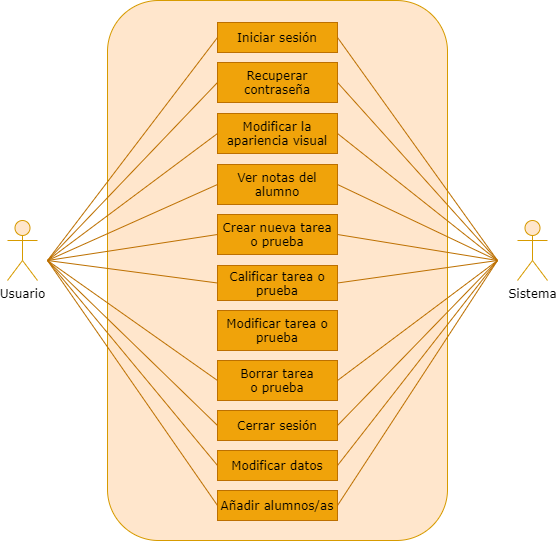
\includegraphics[width=0.75\linewidth]{figs/diagramacdu.png}
\caption{Diagrama de casos de uso de la aplicación.}
\label{Fig:diagramacdu}
\end{figure}

\newpage
\section{\textit{Sprints}}

A continuación se detallan los \textit{sprints} que se realizaron en el proyecto. Hay que indicar que este documento se escribió al mismo tiempo que se iban desarrollando.

\subsection{Primer \textit{sprint}}

En esta iteración se realizó el primer diseño de la base de datos, como ilustra la figura \ref{Fig:db_definition1} y los primeros bocetos de la aplicación, tal y como ilustran la figura \ref{Fig:mockup_mainwindow}. Se pueden encontrar más figuras con los bocetos de la aplicación en el Anexo A, sección \ref{ana:bocetos}. Estos bocetos se han modificado varias veces durante este primer \textit{sprint}.

%\begin{center}
%  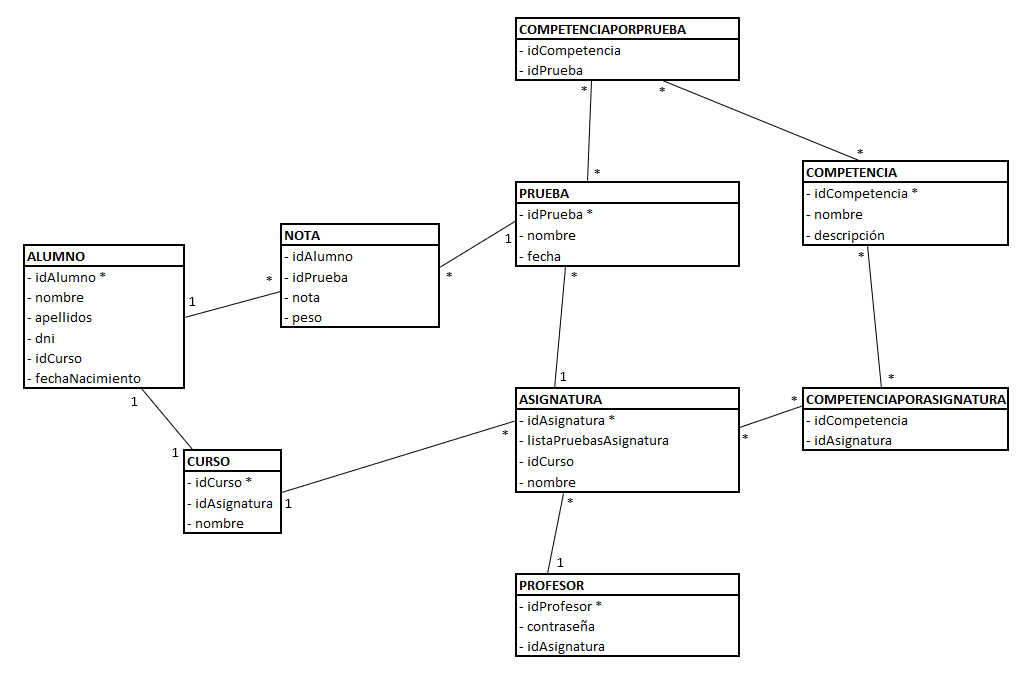
\includegraphics[width=1\linewidth]{figs/DB_Definition_1.png}
%\captionof{figure}{Primera definición de la base de datos.}\label{Fig:db_definition1}%      only if needed  
%\end{center}

\begin{figure}[h]
\centering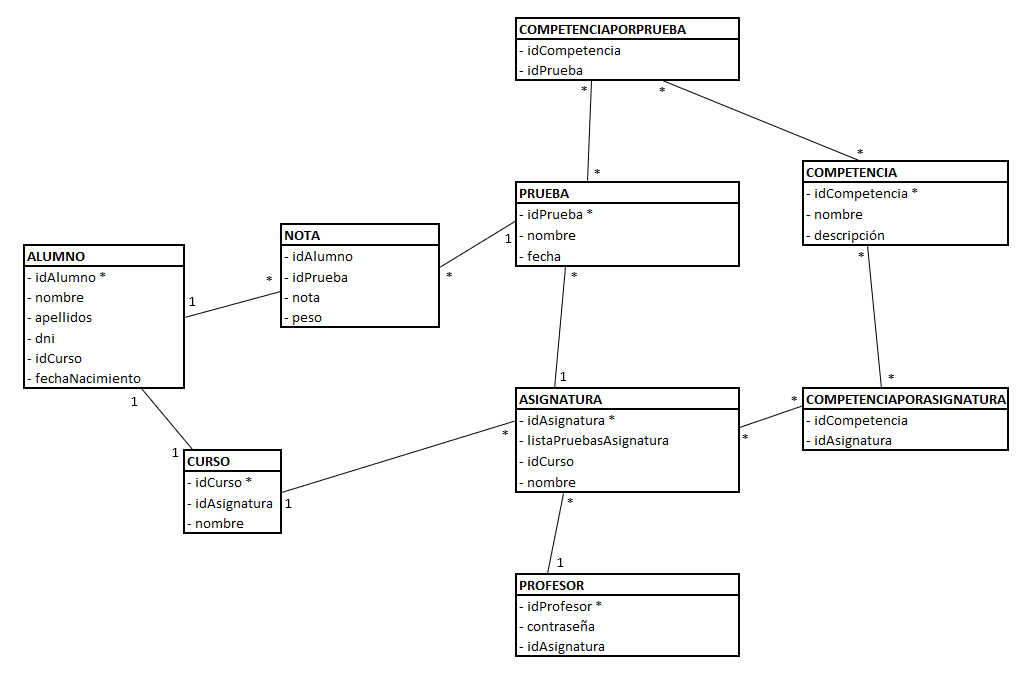
\includegraphics[width=1\linewidth]{figs/DB_Definition_1.png}
\caption{Primera definición de la base de datos.}
\label{Fig:db_definition1}
\end{figure}

%\begin{center}
%  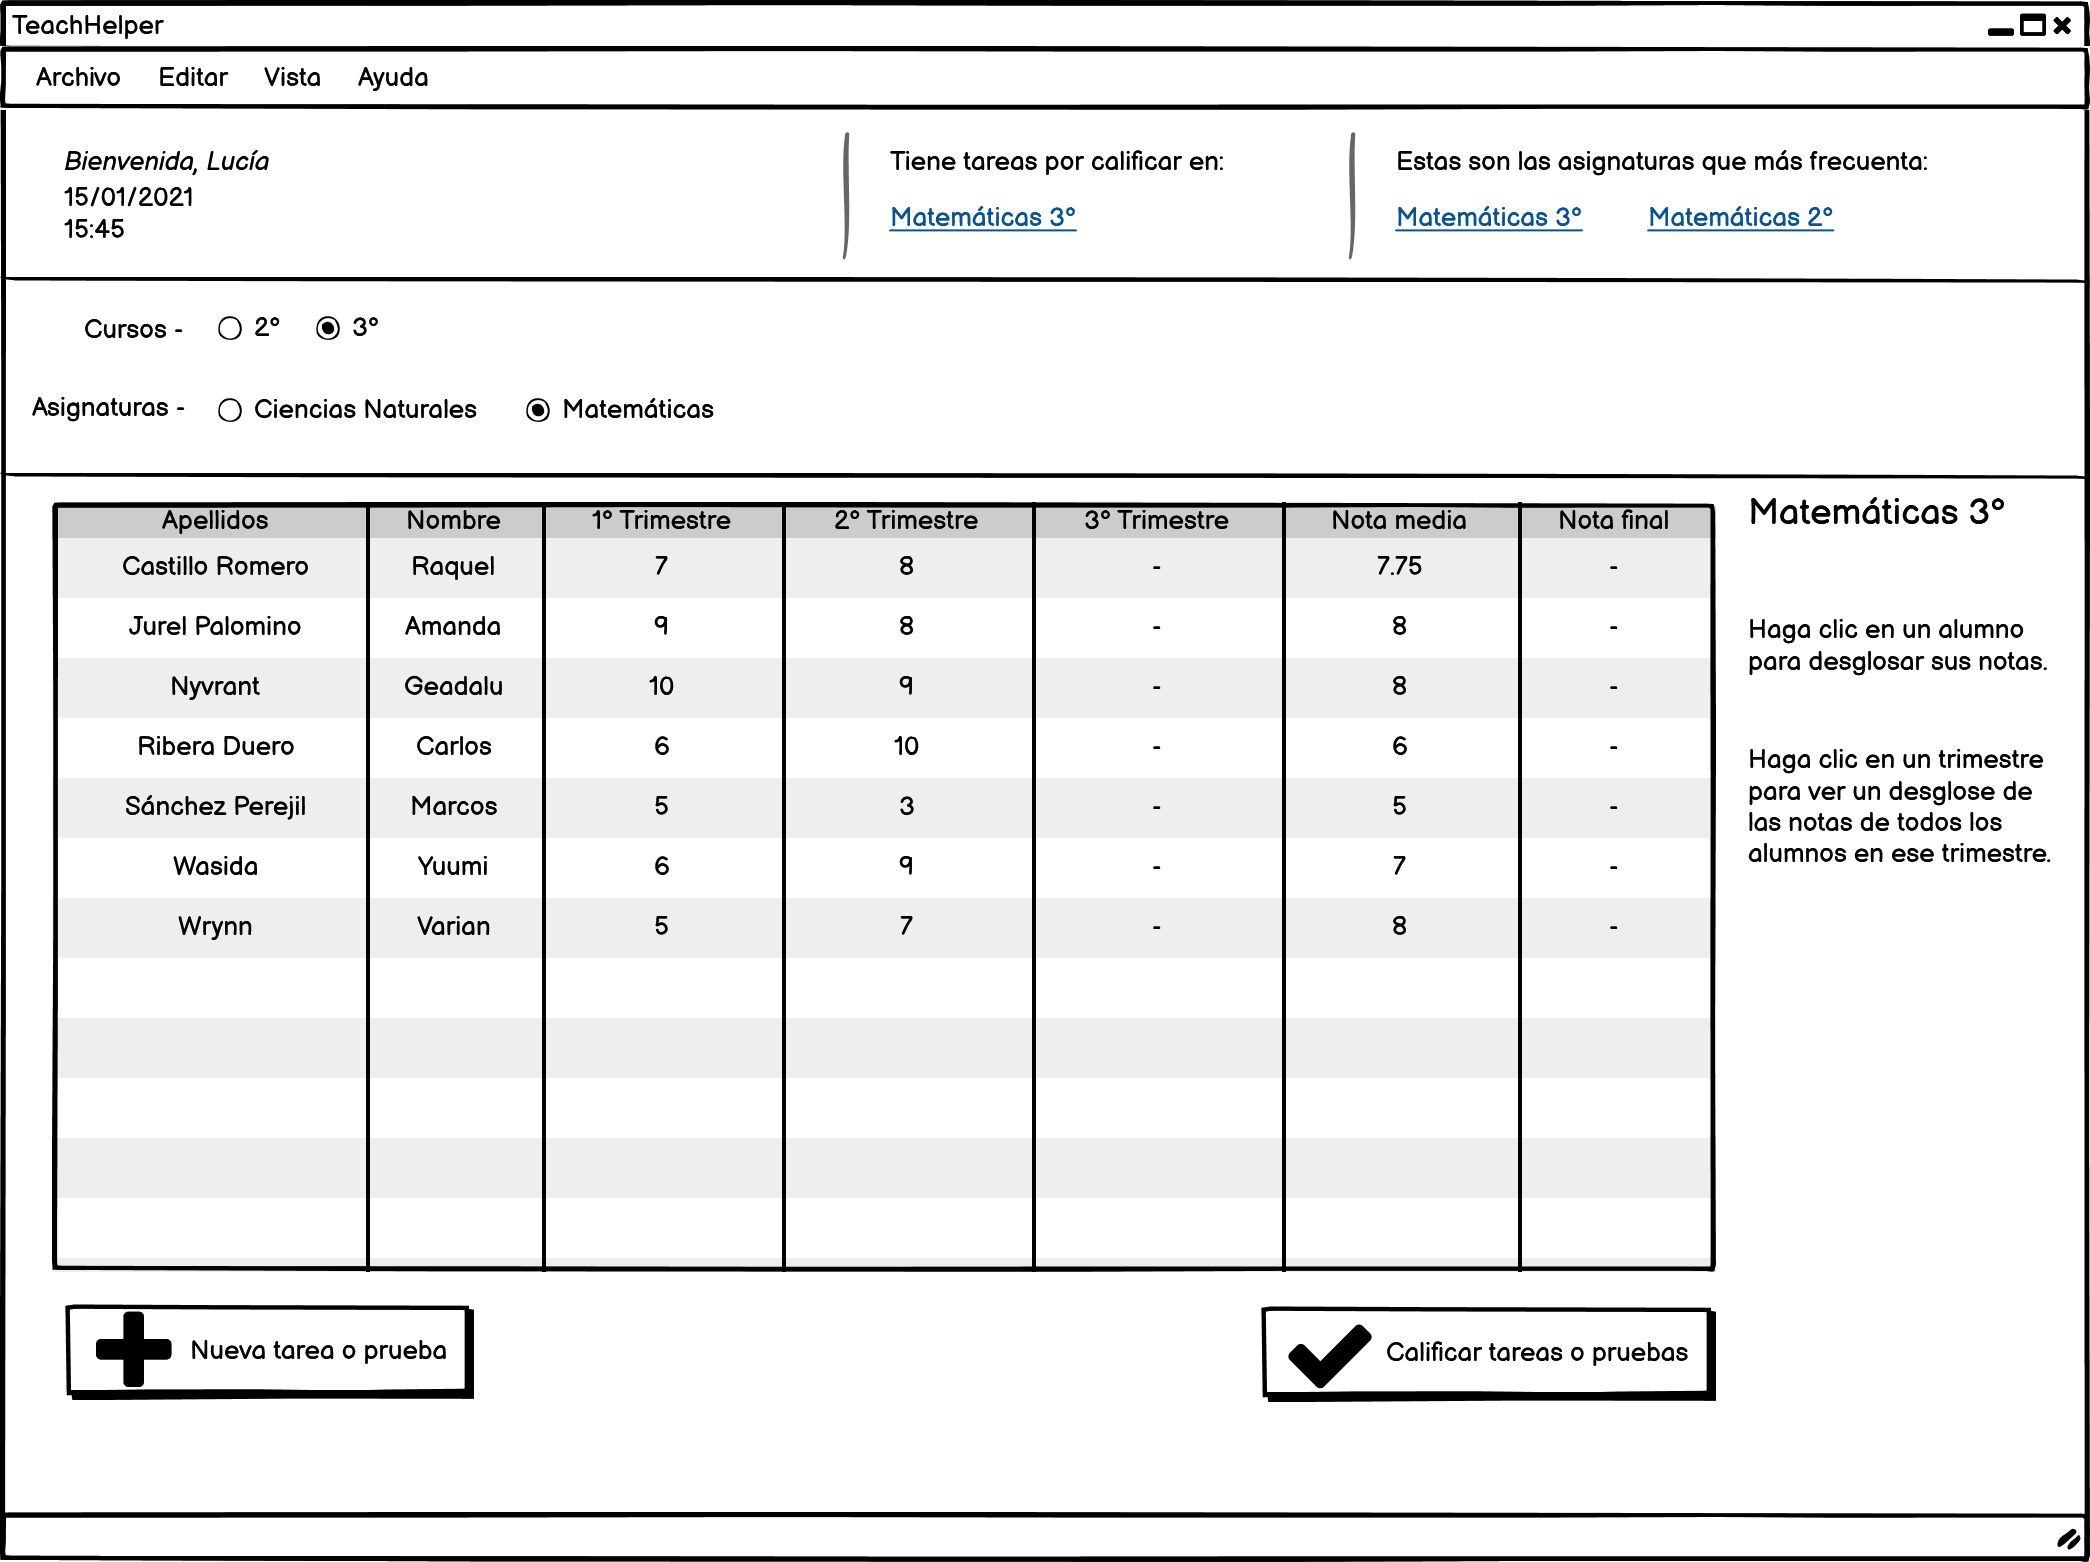
\includegraphics[width=1\linewidth]{figs/mockup_mainwindow.png}
%\captionof{figure}{Prototipo de la ventana principal.}\label{Fig:mockup_mainwindow}%      only if needed  
%\end{center}

\begin{figure}[h]
\centering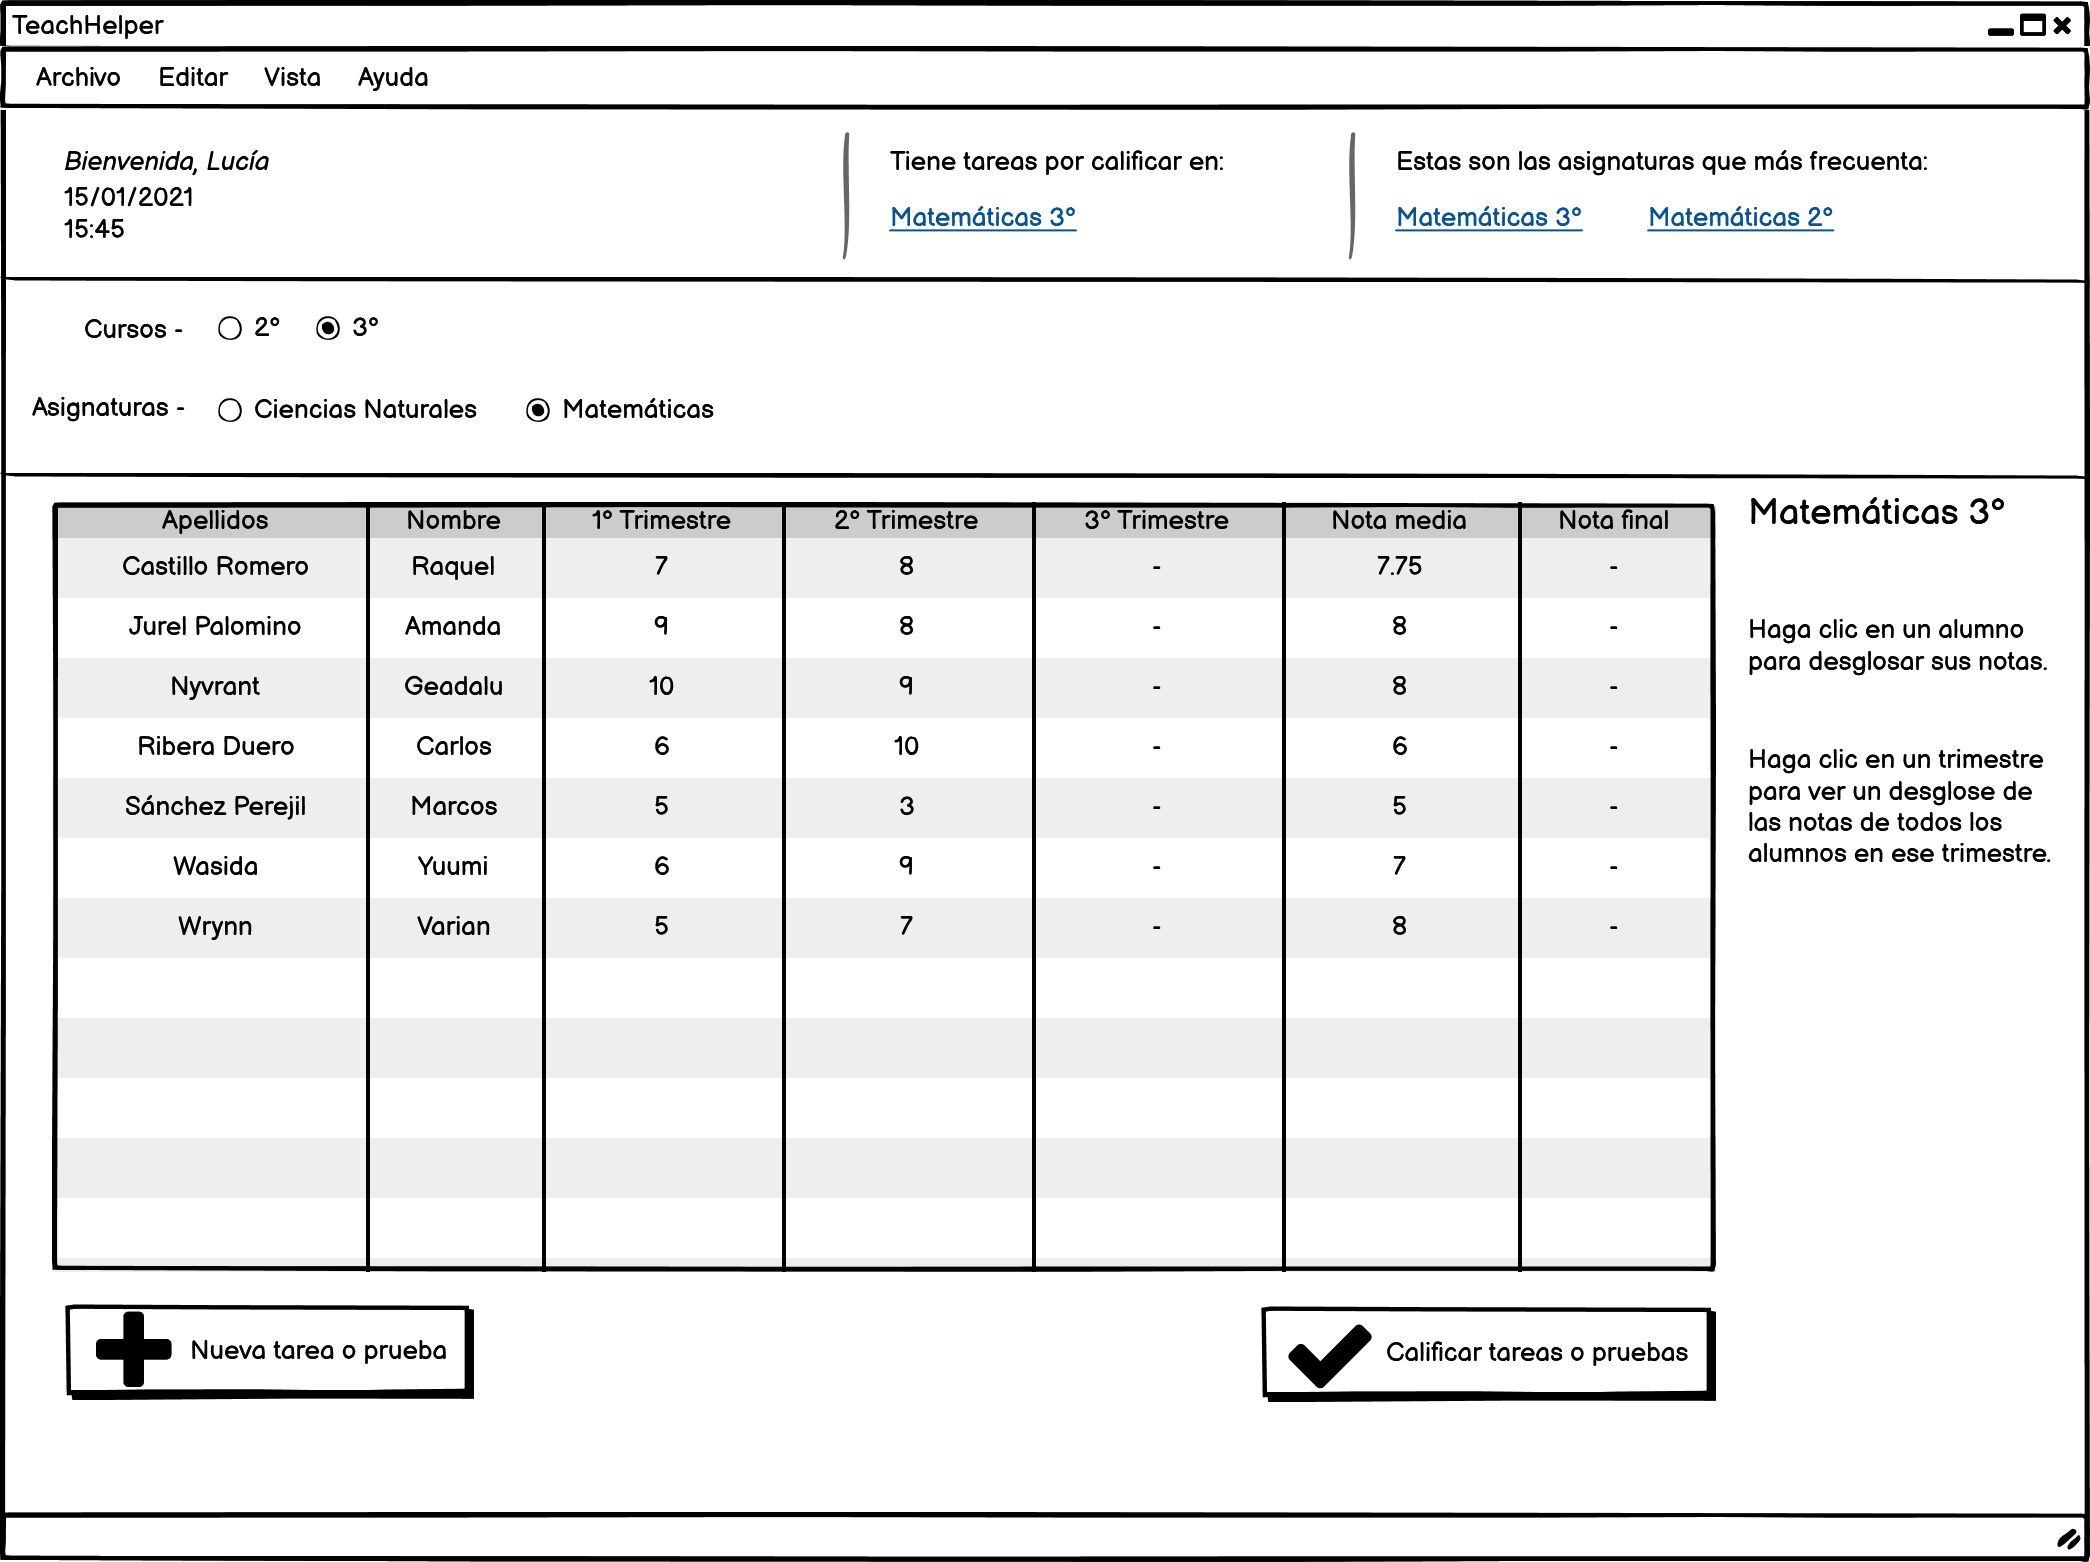
\includegraphics[width=1\linewidth]{figs/mockup_mainwindow.png}
\caption{Prototipo de la ventana principal.}
\label{Fig:mockup_mainwindow}
\end{figure}


\subsection{Segundo \textit{sprint}}
En el segundo \textit{sprint} se comenzó a escribir la memoria del proyecto, empezando por describir las aplicaciones existentes investigadas.

Se siguió trabajando en el diseño e implementación de la base de datos, y comenzó a poblarse de datos de prueba para comenzar el desarrollo.

En la figura \ref{Fig:db_definition6} se muestra la definición completa y final de la base de datos de la aplicación. Se puede ver todo el histórico de modificaciones a la base de datos en el Anexo A, sección \ref{ana:db}.

\begin{figure}[h]
\centering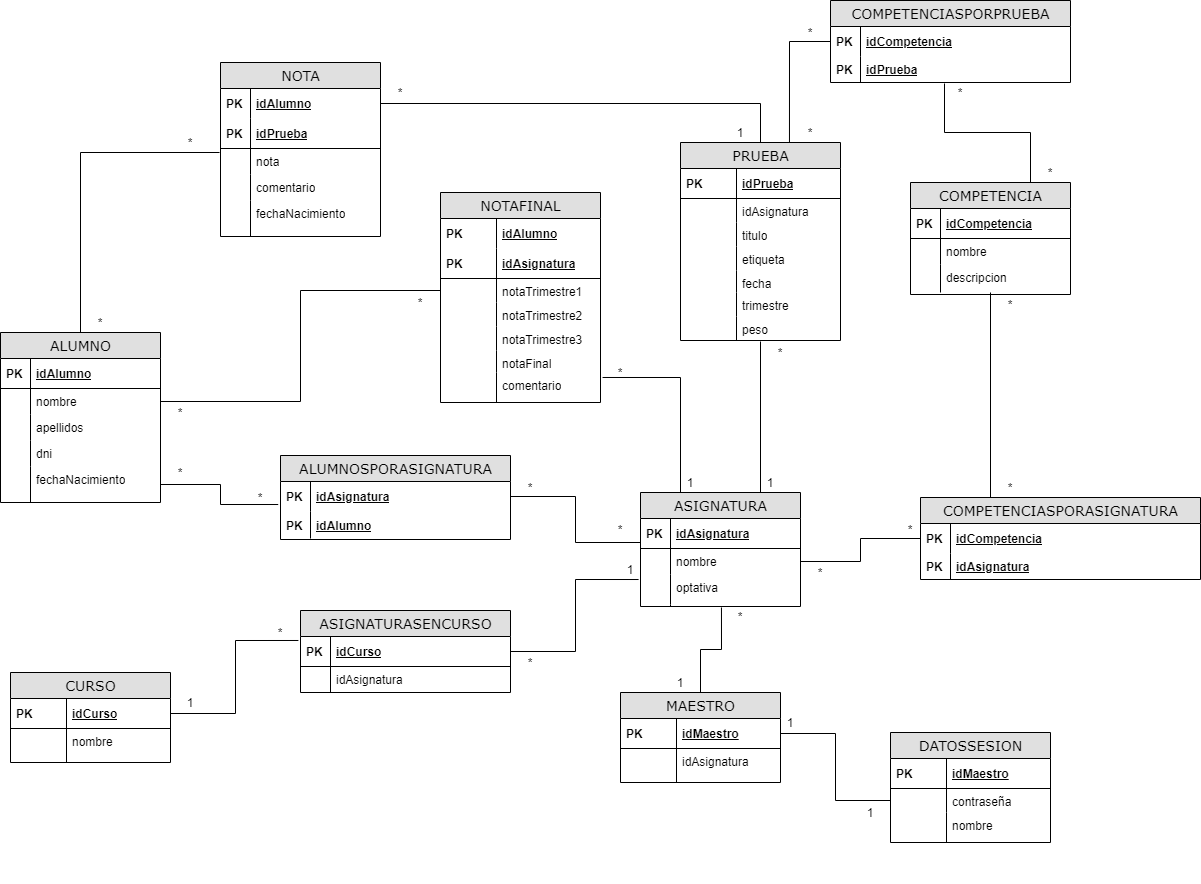
\includegraphics[width=1\linewidth]{figs/DB_Definition_6.png}
\caption{Definición final de la base de datos.}
\label{Fig:db_definition6}
\end{figure}


\subsection{Tercer \textit{sprint}}
En el tercer \textit{sprint} se comenzó la implementación de la aplicación por la ventana principal, debido a que al estar unida a todas las funcionalidades del sistema, se consideró la más importante.

Al final de este sprint se decidió cambiar de \gls{ide} debido a la gran dificultad para trabajar con interfaces en Java con el elegido inicialmente.

\subsection{Cuarto \textit{sprint}}
En el cuarto \textit{sprint} se continuó con el desarrollo de la ventana principal. Cabe notar que en esta iteración se decidió dejar las mejoras del diseño de la ventana para sprints posteriores y comenzar con el desarrollo de las funcionalidades principales:
\begin{itemize}
	\item \textbf{Crear una nueva tarea o prueba}, accesible mediante un botón en la ventana principal.
	\item \textbf{Calificar tareas o pruebas}, accesible de la misma manera, con un botón en la ventana principal.
	\item \textbf{Ver informe del alumno}, ventana que se puede acceder al hacer clic en el nombre de un alumno en la tabla.
	\item \textbf{Ver informe del trimestre}, ventana que se puede acceder al hacer clic en el título de un trimestre en la tabla.
\end{itemize}


Al final de este \textit{sprint}, se comprobó que las funcionalidades desarrolladas se integraban y funcionaban correctamente entre ellas y la ventana principal.

\subsection{Quinto \textit{sprint}}
En el quinto \textit{sprint} se realizaron pequeños desarrollos en la aplicación, tanto para añadir nuevas funcionalidades de los apartados de requisitos \textit{Could have} y \textit{Won't have}, como para pulir las ya existentes.

En este sprint se desarrollaron las siguientes funcionalidades y se hicieron varios arreglos:
\begin{itemize}
	\item \textbf{Modificación de los datos del docente}, accesibles mediante un botón en la ventana principal.
	\item \textbf{Manual de ayuda}, una pequeña ventana con texto explicando al usuario cada funcionalidad de la aplicación. Es accesible mediante cualquier ventana.
	\item \textbf{Añadir alumnos}, funcionalidad posible mediante un formulario, para un solo alumno, o subiendo un Excel, para varios. Accesible mediante la ventana principal.	
\end{itemize}

Durante este periodo de tiempo también se diseñaron las imágenes e iconos usados en la aplicación.

Por último, en este sprint se decidió implementar las estadísticas para las notas en la ventana principal y la ventana de calificar tareas.

\subsection{Temporalización}
Este proyecto, que ha tenido una duración aproximada de 350 horas, se ha desarrollado desde el 2 de octubre de 2020 hasta el 1 de julio de 2021. Se puede ver una tabla con la organización temporal en la figura \ref{Fig:timeline}.

A continuación se desglosan los \textit{sprints} junto con las horas que duró cada uno:
\begin{itemize}
	\item \textbf{Primer sprint:} comenzó el 1 de octubre y terminó el 1 de noviembre, durando 30 horas.
	\item \textbf{Segundo sprint:} comenzó el 2 de noviembre y terminó el 1 de diciembre, durando 20 horas.
	\item \textbf{Tercer sprint:} comenzó el 2 de diciembre y terminó el 1 de febrero, durando 50 horas.
	\item \textbf{Cuarto sprint:} comenzó el 2 de febrero y terminó el 1 de mayo, durando 175 horas.
	\item\textbf{ Quinto sprint:} comenzó el 2 de mayo y terminó el 1 de julio, durando 75 horas.
\end{itemize}

\begin{figure}[H]
\centering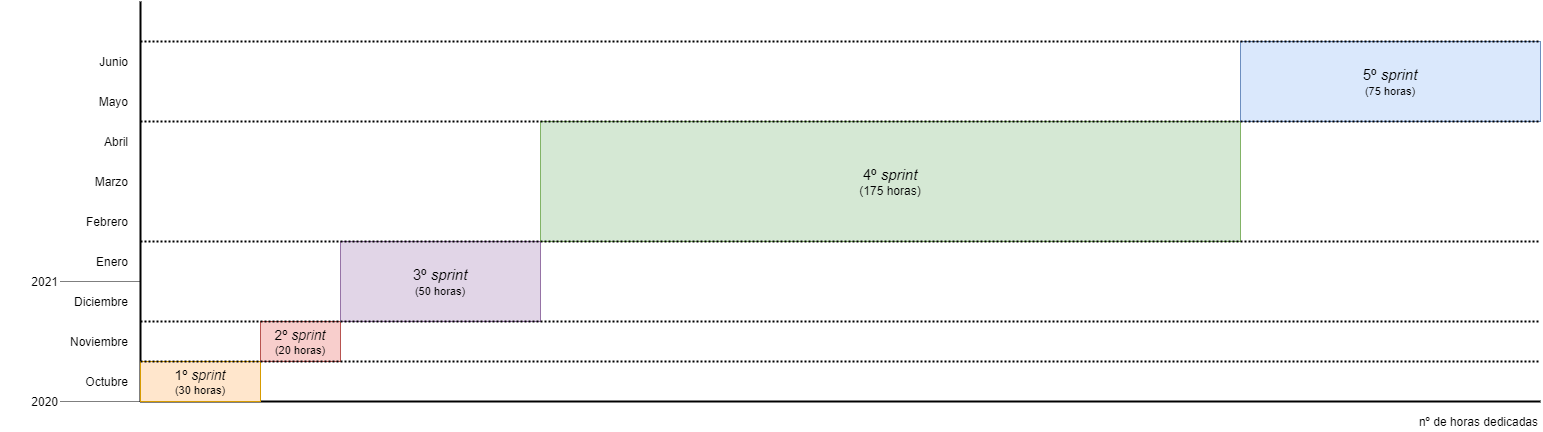
\includegraphics[width=1\linewidth]{figs/timeline.png}
\caption{Organización temporal del proyecto.}
\label{Fig:timeline}
\end{figure}

\section{Resultado del desarrollo}
En esta sección se muestra la solución propuesta hablando de su diseño y su implementación.
En el Anexo A se pueden encontrar diagramas de secuencia de los casos de uso más interesantes, y en el Anexo D, un Manual de usuario de la aplicación, mostrando capturas de cada ventana y explicando todos los procesos que se pueden llevar a cabo.

\subsection{Arquitectura y diseño de la aplicación}

\subsubsection{Estructura externa}
Para diseñar la arquitectura de la aplicación se ha optado por un modelo mixto Vista-Controlador, donde las capas que contienen los controladores y los objetos se conectan con la base de datos, y la capa con las interfaces, hace llamadas a los controladores y objetos para operar con ella.

\begin{figure}[H]
\centering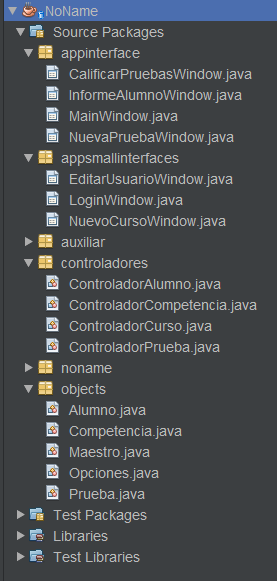
\includegraphics[width=0.25\linewidth]{figs/arquitectura.png}
\caption{Arquitectura del código siguiendo un modelo mixto Vista-Controlador.}
\label{Fig:arquitectura}
\end{figure}

\begin{itemize}
	\item \textbf{Capa de vistas:} representa las interfaces del programa: los paquetes asociados a esta capa son \textit{appinterface} y \textit{appsmallinterfaces}.
	\item \textbf{Capa de controladores:} se comunica con la base de datos y hace operaciones utilizando la capa de objetos. El paquete \textit{controladores} es el que representa esta capa.
	\item \textbf{Capa de objetos:} se comunica con la base de datos, contiene todos los objetos del programa. Es representada mediante el paquete \textit{objects}.
\end{itemize}

Se es consciente de que, si fuera un modelo vista-controlador puro, los controladores no deberían acceder a la base de datos. Esto se ha realizado para, entre otras cosas, permitir una mayor comprensión del código debido a que los métodos de los controladores que realizan operaciones en la base de datos, lo hacen siempre sobre una lista de objetos, mientras que los métodos de los propios objetos que tienen similar propósito, lo realizan solo sobre el objeto en sí. De esta manera, un método que quiera actualizar las notas de todos los alumnos de una asignatura se encontrará en el controlador, y uno que quiera actualizar el nombre del docente, se encontrará en la clase que representa al docente.

\subsubsection{Estructura interna}

Atendiendo a los requisitos recogidos, se propuso la estructura de la figura \ref{fig:diagramaclases} como diagrama de clases para la aplicación.
%Añadir diagrama de clases.

\begin{sidewaysfigure}[]
  \centering
  \caption{Diagrama de clases de la aplicación.}
  \label{fig:diagramaclases}
  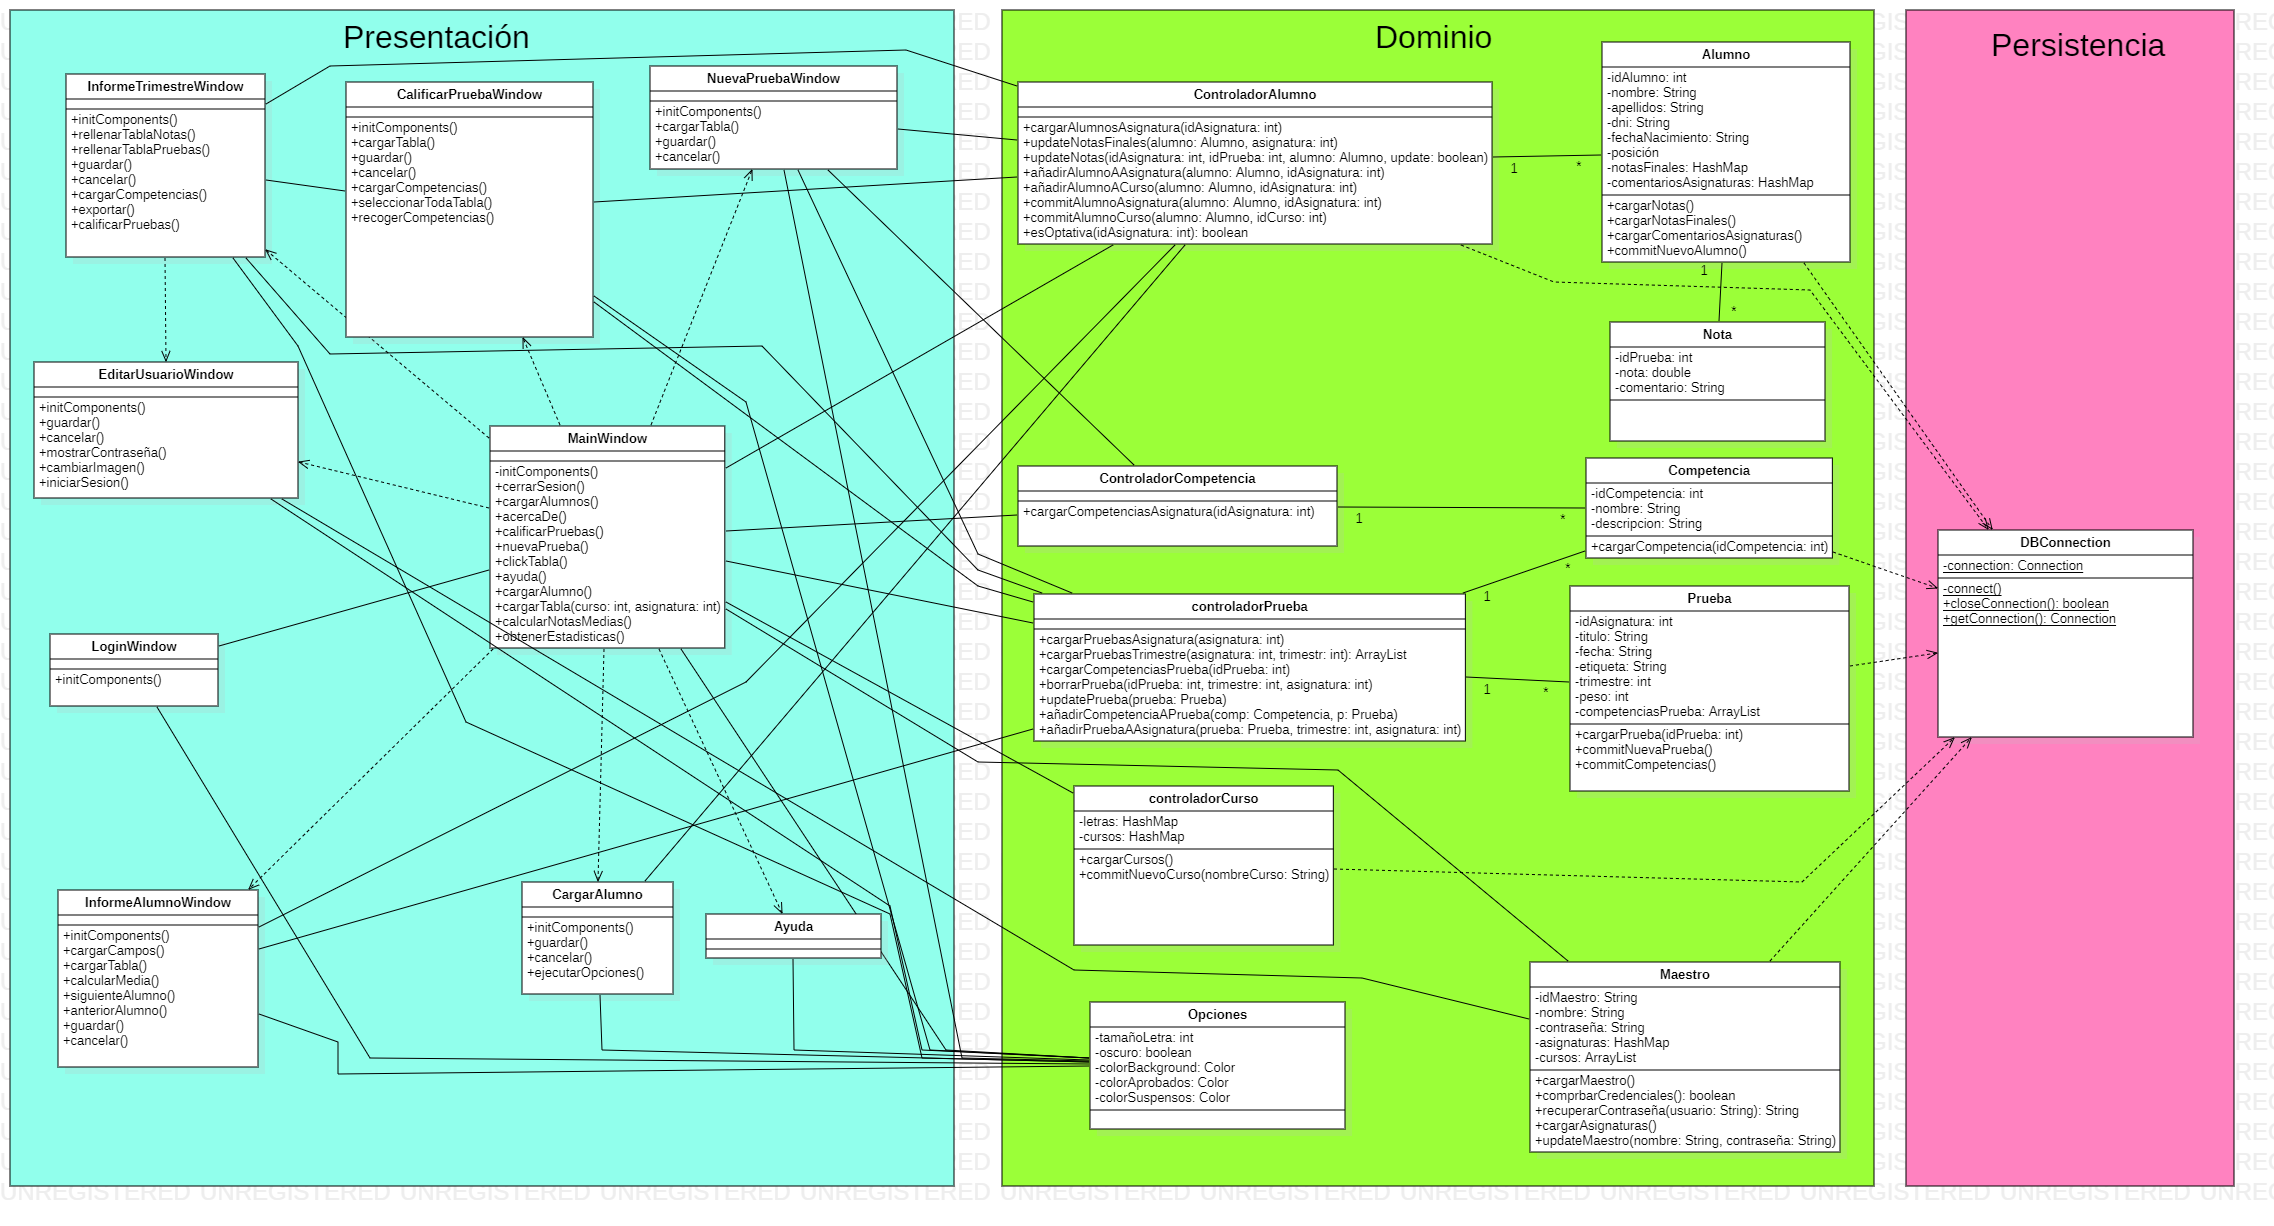
\includegraphics[width=1\linewidth]{figs/ClassDiagram.png}
\end{sidewaysfigure}

Como se puede observar, se sigue una estructura en capas:
\begin{itemize}
\item\textbf{Presentación}. Esta capa posee las interfaces de la aplicación. Se correspondería con la capa de vistas de la estructura externa.
\item\textbf{Dominio}, donde están las clases que dan las funcionalidades al programa y las que se comunican con la capa de persistencia. Esta capa se correspondería con las capas de objetos y controladores de la estructura externa.
\item\textbf{Persistencia}, la capa que posee la conexión con la base de datos.
\end{itemize}

Se puede ver con más detalle en el Anexo A, sección \ref{ana:clases}.



\subsection{Implementación}
\label{sub:implementacion}
Este proyecto, desarrollado en Java, es compatible con cualquier sistema operativo.

Esta sección se dedicará a comentar el código escrito para desarrollar la aplicación, haciendo hincapié en los aspectos algorítmicos y mostrando fragmentos de código interesantes para la solución.

\subsubsection{Estructuras de datos}
Se han utilizado las siguientes estructuras de datos de Java para gestionar los datos de la solución:

\textbf{Diccionarios}: se ha primado el uso de diccionarios (pares clave/valor) como estructura principal de almacenamiento de datos, en concreto de los \textit{HashMaps}, la estructura de diccionario de Java más rápida para el alcance del problema\cite{hashmap}.

El tiempo de acceso de las operaciones añadir, borrar y buscar es \textit{O(1)}. Estas son las operaciones que se han usado en el código. De hecho, la única casuística en la que un \textit{HashMap} puede dar problemas de rendimiento es si tiene demasiados datos dentro: las operaciones se volverían más lentas. Esto también se ha evitado en la solución propuesta, donde el número máximo de elementos de cualquiera de estas estructuras es el número de alumnos y alumnas en una asignatura.

\textbf{Listas}, que en Java se corresponden con la estructura \textit{ArrayList}. Estas listas se han utilizado para almacenar los objetos Java que contienen los datos de la base de datos, por ejemplo, una lista de alumnos y alumnas.

La parte interesante de usar estas dos estructuras de datos es la combinación que se ha logrado entre ellas, de tal forma que la lista del alumnado mencionada anteriormente se convertiría en la lista del alumnado de una asignatura en específico, al meterla dentro de un diccionario:
 
\begin{lstlisting}
private HashMap<Integer, ArrayList<Alumno>> alumnosAsignatura;
\end{lstlisting}

El parámetro \textit{integer}, clave del diccionario, es el código de la asignatura y el ArrayList<Alumno>, el valor, la lista de alumnos y alumnas que pertenecen a dicha asignatura.

La estructura más compleja que se ha manejado en el proyecto ha sido la que almacena las pruebas de cada asignatura, debido a que debían estar organizadas, además, por trimestres. Esto se consiguió mediante la siguiente combinación de diccionarios y listas:

\begin{lstlisting}
private HashMap<Integer, HashMap<Integer, ArrayList<Prueba>>> pruebasAsignatura;
\end{lstlisting}

Este diccionario \textit{pruebasAsignatura} contiene, por cada clave, otro diccionario con la lista de pruebas de cada trimestre, de tal forma que se accede primero a la asignatura, y luego al trimestre (mediante el segundo diccionario) para sacar su lista de pruebas.

Las estructuras de datos del código fueron modificadas numerosas veces a lo largo del proceso de desarrollo debido a los requerimientos de las funcionalidades nuevas de cada \textit{sprint}. Esto supuso un esfuerzo que no estaba contemplado e impactó de manera negativa en el cuarto \textit{sprint}, que duró 20 horas más de las previstas.

A continuación se habla del algoritmo que más cambios ha sufrido en el desarrollo de la aplicación: el que guarda las notas en la base de datos desde la ventana del informe del alumno.

\begin{lstlisting}
public void guardarNotas() {
        model1 = (DefaultTableModel) tabla1.getModel();
        model2 = (DefaultTableModel) tabla2.getModel();
        model3 = (DefaultTableModel) tabla3.getModel();
        ArrayList<Nota> notas = contAlumnos.getAlumnosAsignatura().get(asignatura)
        .get(alumno.getPosicion()).getNotas();
        updateNotas(model1, notas);
        updateNotas(model2, notas);
        updateNotas(model3, notas);

        //Guardar notas finales
        ArrayList<Double> notasFinales = contAlumnos.getAlumnosAsignatura().get(asignatura)
        .get(alumno.getPosicion()).getNotasFinales().get(asignatura);
        if (notasFinales == null) { //si no tiene todavía notas finales
            notasFinales = new ArrayList<>();
            
            
            if (final1.getText().equals("")) {
                notasFinales.add(0.0);
            } else {
                notasFinales.add(Double.parseDouble(final1.getText()));
            }
            
             //aquí se repiten las 5 últimas líneas de código para los tres trimestres y la nota final
             {...}

            
            //se copian las notas finales desde el hashmap para sustituirlo por las nuevas
            HashMap<Integer, ArrayList<Double>> todasNotasFinales = contAlumnos.getAlumnosAsignatura().get(asignatura)
            .get(alumno.getPosicion()).getNotasFinales();
            todasNotasFinales.put(asignatura, notasFinales);
            contAlumnos.getAlumnosAsignatura().get(asignatura)
            .get(alumno.getPosicion()).setNotasFinales(todasNotasFinales);

        } else {
            if (final1.getText().equals("")) {
                notasFinales.add(0.0);
            } else {
                notasFinales.set(0, Double.parseDouble(final1.getText()));
            }

            //aquí se repiten las 5 últimas líneas de código para los tres trimestres y la nota final
            {...}
            
        }

        //aquí añadimos o modificamos el comentario de la asignatura
        {...}

        try {
            contAlumnos.updateNotasFinales(alumno, asignatura);
        } catch (SQLException e) {
            AuxiliarMethods.showWarning("Ha ocurrido un error al guardar las notas de los alumnos.\nMás información: " + e.toString());
        }
    }
\end{lstlisting}

Los cambios sufridos por este algoritmo se deben a que las notas finales nuevas estaban vacías y tenían que ser creadas en el propio programa para, más tarde, ser almacenadas en la base de datos. Se probó creándolas como vacías (tanto ''\textit{null}'' como cadena vacía), así como asignándoles un valor imposible (-1), pero finalmente se decidió hacerlo con 0, ya que en \gls{eso} no está permitido calificar a un alumno con un 0 en la nota final de un trimestre, por lo que todas las notas que vinieran de la base de datos como 0, no se mostrarían y se quedarían vacías.

A este problema se le sumaba el hecho de que había que diferenciar, a la hora de guardar en la base de datos, si era una creación de una nueva ocurrencia o una actualización. La diferencia principal era si, dentro del programa, cualquier nota había pasado a ser distinta de 0, o todas las notas de los 3 trimestres eran 0.

Para resolver esto, se decidió dividir el algoritmo en esas dos casuísticas: 

\textbf{1.} El alumno no tiene todavía calificado ningún trimestre.
En este caso, hay que crear una estructura de datos para almacenar las notas que se van a recoger.

\textbf{2.} El alumno tiene calificado uno o más trimestres.
Se modifica la estructura de datos ya existente con las notas nuevas.

Gracias a esta solución, se consigue ahorrar, para la recogida de la nota de cada trimestre, una llamada a la lista de las notas finales de cada alumno para comprobar si está vacía.

Al final, desde el controlador de los alumnos se escriben en la base de datos las notas nuevas.


\subsection{Decisiones de diseño e implementación}
En esta sección se describirán algunas de las decisiones que se han tomado respecto al diseño de la aplicación que pueden ser de interés.

\textbf{Procedencia de los iconos e imágenes de la aplicación}.
Los iconos de una aplicación son un arma de doble filo: pueden guiar al usuario por las tareas que quiere realizar, o confundirlo si la funcionalidad asociada al icono no es clara o, directamente, es incoherente.

Para implementar iconos en esta aplicación se han decidido usar las convenciones de las aplicaciones modernas: una imagen de un disquete para los botones de guardar, una cruz roja para cancelar, un icono de encendido para cerrar sesión, un engranaje para acceder a las opciones de configuración, etc. Algunos ejemplos pueden verse en la figura \ref{Fig:iconosusados}.

\begin{figure}[h]
\centering
\includegraphics[width=0.5\linewidth]{figs/iconosusados.png}
\caption{Iconos convencionales usados en la aplicación.}
\label{Fig:iconosusados}
\end{figure}

Sin embargo, para las funcionalidades específicas, se han diseñado la mayoría de los iconos e imágenes mediante la aplicación Procreate. Los iconos que no se han diseñado y se han descargado de Internet han sido el disquete\cite{disquete}, el icono de Microsoft Excel\cite{excelicon} y el icono de la papelera\cite{iconsforfree}.

\textbf{Opciones especiales para personas con daltonismo}.
A la hora de implementar las opciones de colores para la interfaz, accesibles mediante la ventana de inicio de sesión, ha sido muy importante tener en cuenta todas las combinaciones de colores de manera que, aun eligiendo tonos parecidos, se pudiera seguir leyendo correctamente.

La prueba con diferentes tonalidades llevó a pensar que, efectivamente, hay personas que no distinguen bien colores que, a primera vista, son muy diferentes, como pueden ser el verde y el rojo asignados a las calificaciones aprobado y suspenso, respectivamente. Esta condición se llama daltonismo, que es una alteración de origen genético que impide identificar correctamente los colores. Uno de los tipos de daltonismo más comunes es la deuteranopia, razón por la cual se incluyó en las opciones de personalización un "modo para daltónicos".

Esta opción especial modifica los colores de aprobados y suspensos para que sean colores fácilmente reconocibles para personas con esta condición (ver figura \ref{Fig:appdaltonicos}).

Para finalizar esta sección, comentar que se hizo una pequeña prueba de usabilidad con una persona daltónica. Se le mostraron primero los colores por defecto y después los colores elegidos para el 'Modo daltónicos'. Afirmó que solo el segundo conjunto de colores era fácilmente distinguible.
\newpage

\begin{figure}[H]
\centering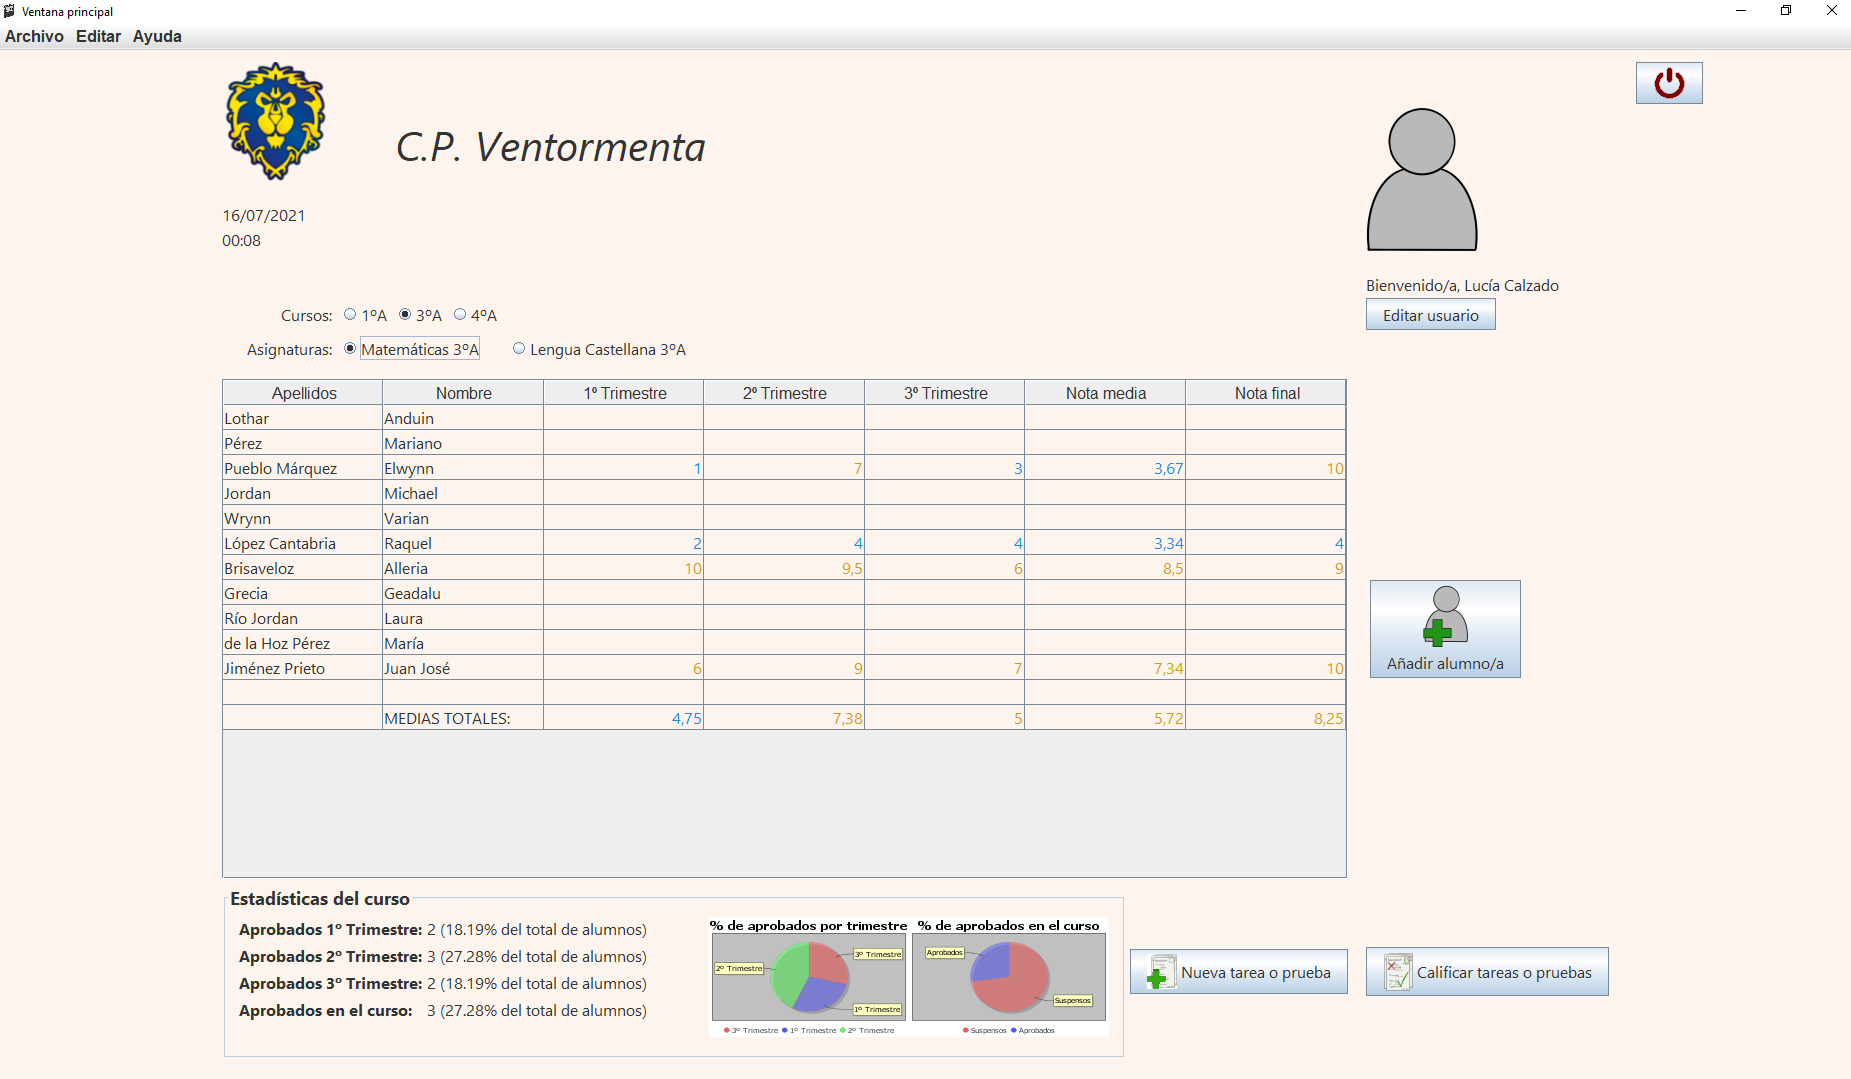
\includegraphics[width=1\linewidth]{figs/appdaltonicos.png}
\caption{Visualización de la pantalla principal con el modo daltónicos activado.}
\label{Fig:appdaltonicos}
\end{figure}

\section{Aplicación obtenida}
El resultado de este desarrollo es una aplicación de escritorio con las siguientes funcionalidades:
\begin{itemize}
	\item \textbf{Identificación:} el docente puede identificarse en la aplicación mediante su DNI y una contraseña.
	\item \textbf{Personalización del perfil} del docente mediante imagen personal y nombre, así como modificación de su contraseña.
	\item \textbf{Personalización de la interfaz} cambiando el color de fondo de la aplicación y los colores de las aplicaciones.
	\item \textbf{Visualización de las notas del alumnado} de varias maneras: filtrando por trimestre, por prueba o por alumno o alumna y acompañadas de estadísticas para mejor visualización.
	\item \textbf{Gestión de las tareas:} se permite crear y borrar tareas dentro de cada asignatura, así como asignarlas a ciertos alumnos o alumnas.
	\item \textbf{Gestión de las calificaciones} del alumnado: se pueden calificar las tareas creadas y los trimestres de cada asignatura.
	\item \textbf{Creación de alumnado nuevo} que cubre las incorporaciones a mitad del curso.
\end{itemize}

En las figuras \ref{Fig:resventanaprincipal} y \ref{Fig:rescalificaciontareas} se pueden ver dos de las ventanas de la aplicación: la ventana principal y la calificación de tareas, respectivamente. El Anexo D corresponde al manual de usuario de la aplicación y en él se pueden ver el resto de ventanas, así como una explicación exhaustiva de las funcionalidades que tiene cada una.

\begin{figure}[H]
\centering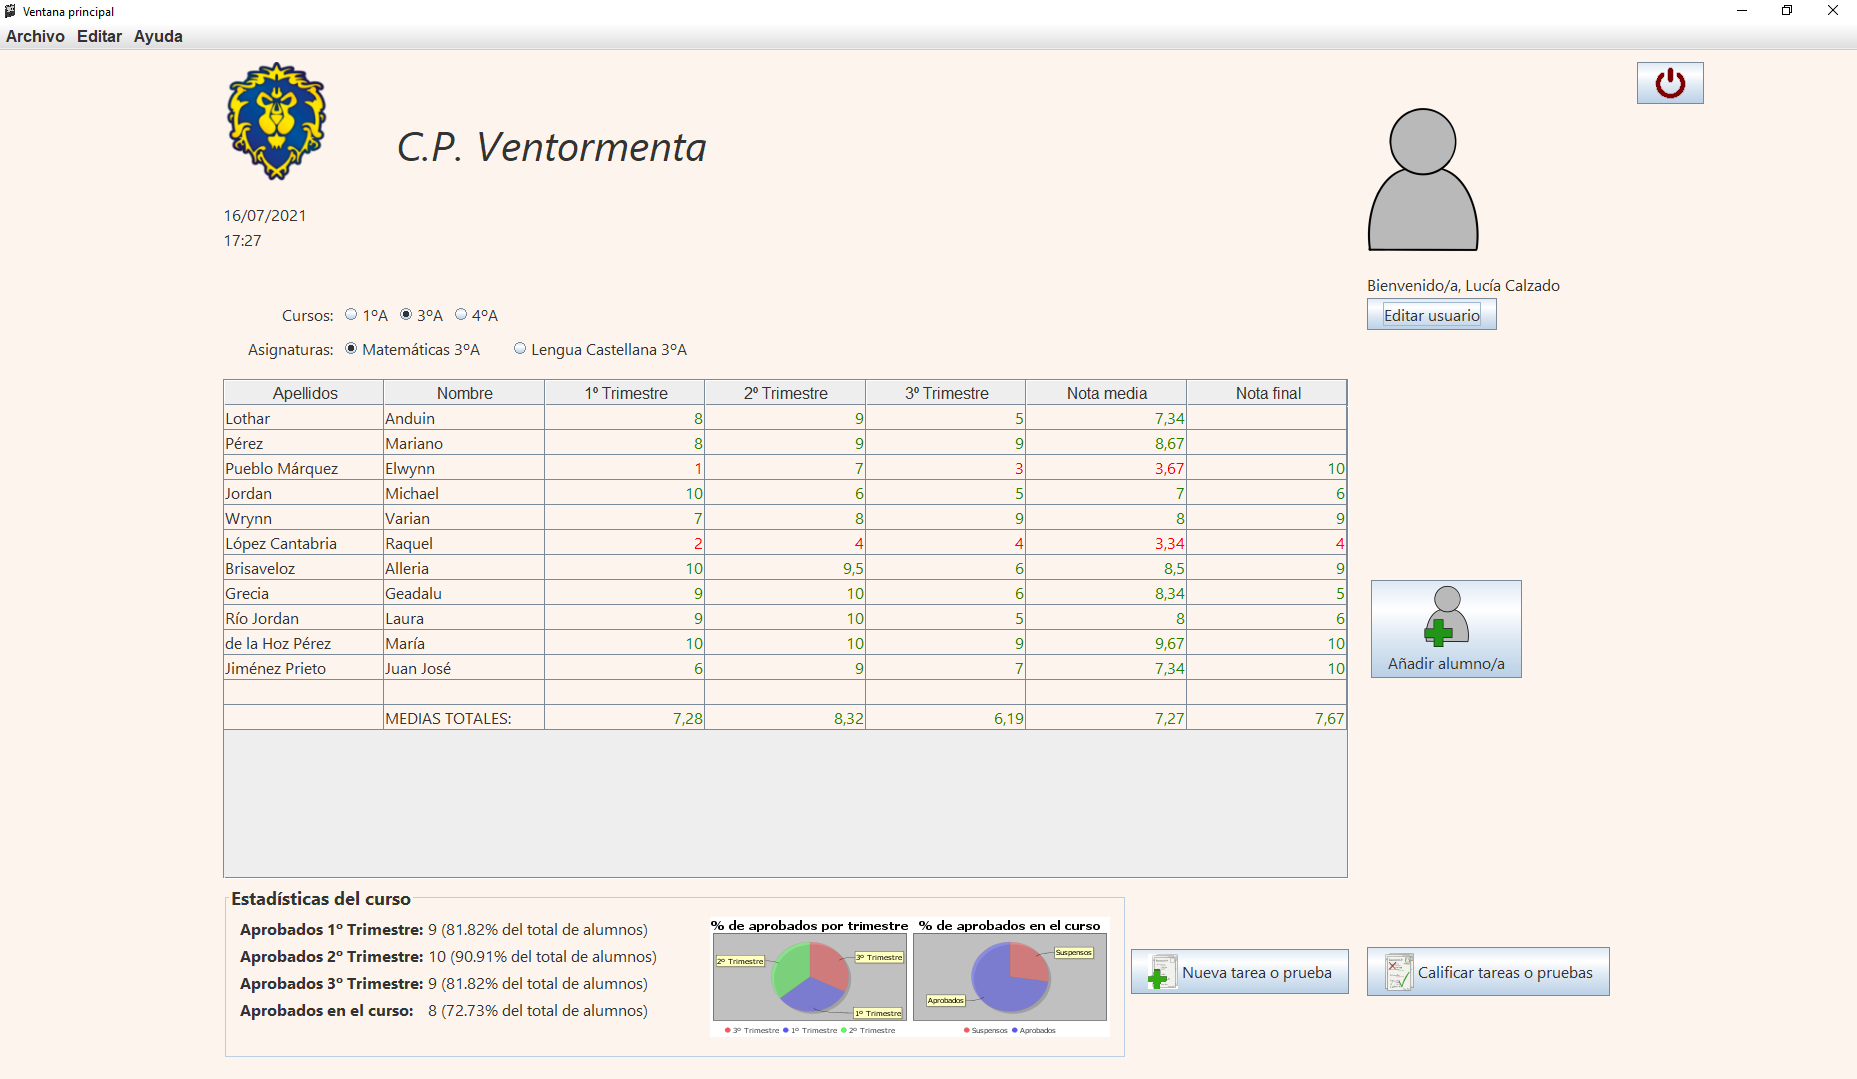
\includegraphics[width=1\linewidth]{figs/ventanaprincipal.png}
\caption{Ventana principal.}
\label{Fig:resventanaprincipal}
\end{figure}

\begin{figure}[H]
\centering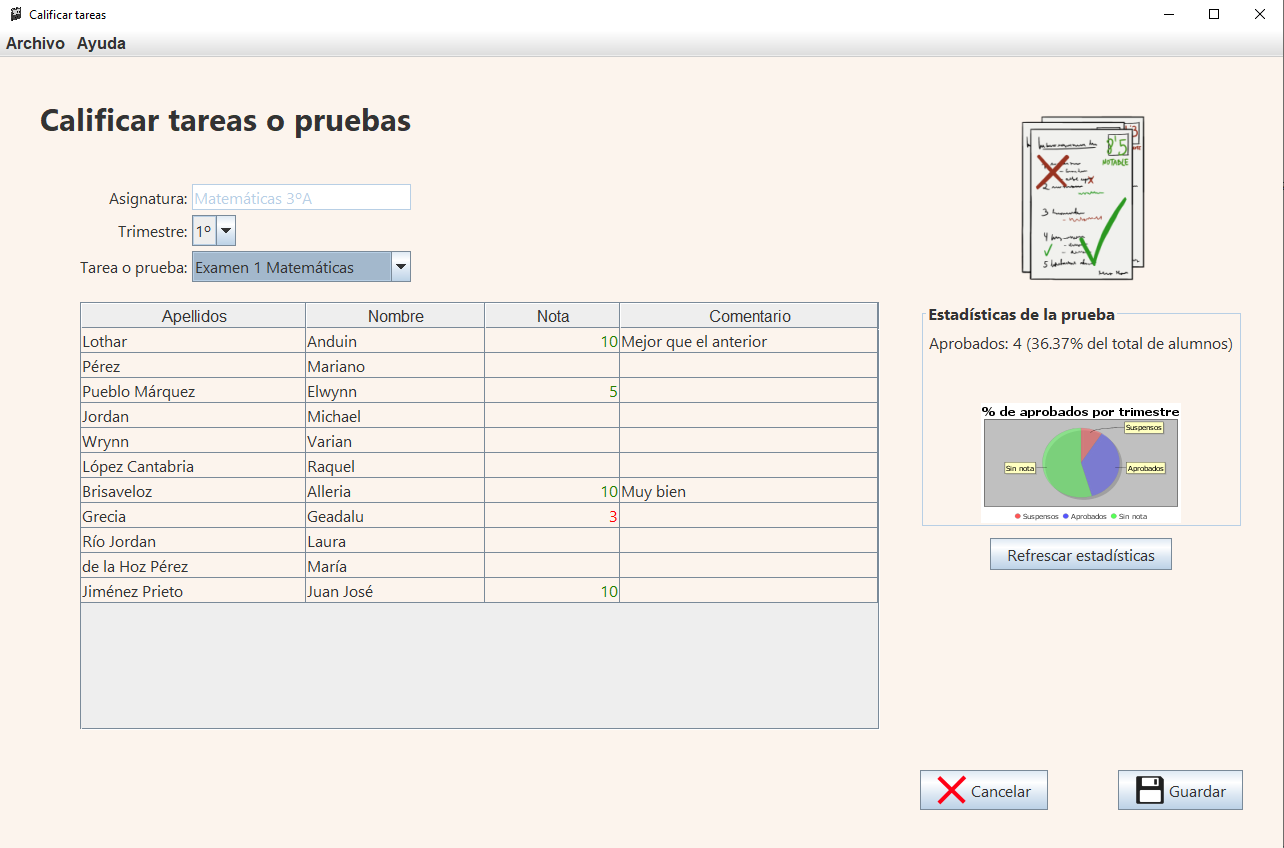
\includegraphics[width=1\linewidth]{figs/calificartareas.png}
\caption{Ventana de calificación de tareas.}
\label{Fig:rescalificaciontareas}
\end{figure}

\newpage

\section{Evaluación del sistema}
\label{sub:pruebausabilidad}
Para comprobar si la aplicación desarrollada cumple las expectativas, los requisitos descritos y si tiene carencias o no, se ha realizado una pequeña experiencia con potenciales usuarios para evaluar su usabilidad.

\subsection{Diseño de la experiencia}
En la experiencia participaron, de forma voluntaria, 34 docentes. Para ello, se les preparó un vídeo explicativo de la aplicación y se les suministró acceso a un formulario, creado en Google Forms, para que, de forma completamente anónima, proporcionasen su opinión sobre la usabilidad de la herramienta y la intención de uso de la misma. El cuestionario consta de 12 ítems, con respuestas en una escala de Likert de cinco niveles, según el grado de acuerdo o desacuerdo con cada uno de ellos, y de tres preguntas de respuesta abierta. Los 8 primeros ítems corresponden a la traducción al castellano de la escala SUS\cite{sus} para medir la usabilidad de herramientas web; los 4 restantes, basados en el \textit{framework} TAM\cite{tam}, miden la intención de uso de la aplicación. Las respuestas abiertas dan la opción al usuario a indicar los puntos fuertes y débiles del sistema, así como opciones de mejora. El contenido completo del cuestionario se puede consultar en el Anexo C.

\subsection{Análisis de los resultados}

El análisis de los resultados, que ilustran las figuras \ref{Fig:pregunta4} y \ref{Fig:pregunta5}, refleja la buena valoración que ha tenido la aplicación.

\begin{figure}[h]
\centering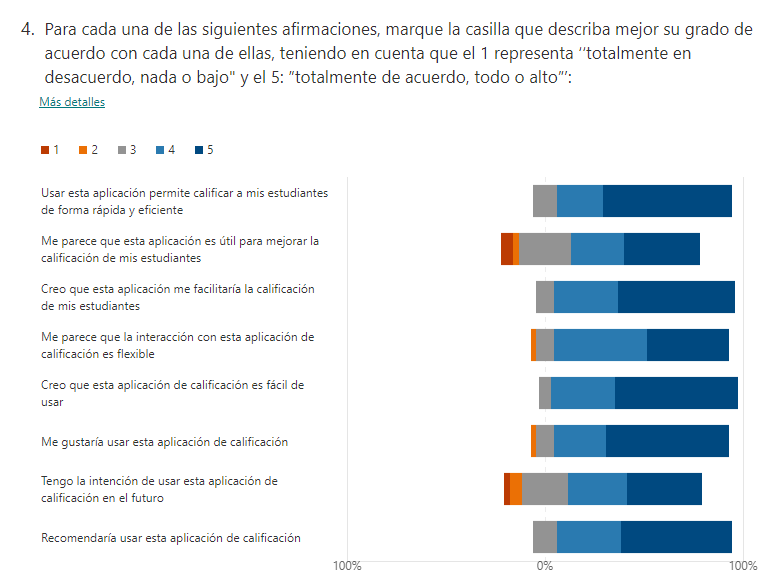
\includegraphics[width=1\linewidth]{figs/pregunta4.png}
\caption{Pregunta 4 del cuestionario.}
\label{Fig:pregunta4}
\end{figure}

\begin{figure}[h]
\centering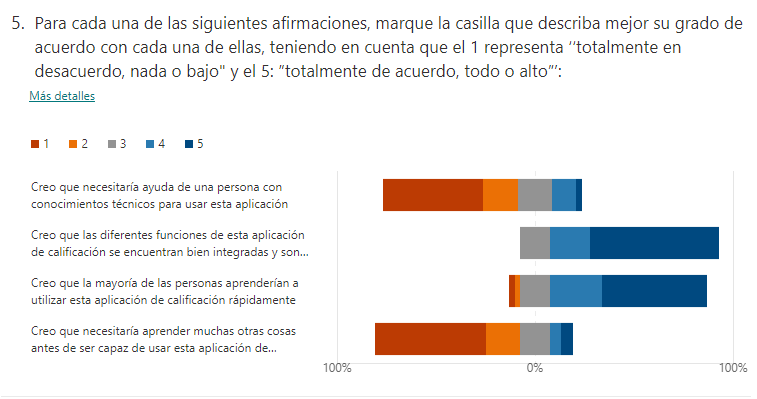
\includegraphics[width=1\linewidth]{figs/pregunta5.png}
\caption{Pregunta 5 del cuestionario.}
\label{Fig:pregunta5}
\end{figure}

A continuación se realiza un pequeño análisis sobre el cuestionario.

Los resultados han sido generalmente favorables. Considerando, en la cuarta pregunta, que un 4 o un 5 son respuestas aceptables, se puede observar que al 64,7\% de los encuestados les parece útil la aplicación desarrollada para mejorar la forma en la que califican a sus estudiantes, y al 88.3\% les gustaría poder llegar a usarla.

En la quinta pregunta también encontramos resultados contundentes. Solo el 11,8\% de los encuestados considera que necesitaría formación previa para usar la aplicación correctamente respecto al 73,5\% que no creen que fueran a tener ningún problema.

Algunos comentarios de los encuestados cuando se les preguntó por los puntos fuertes de la aplicación son:
\begin{quote}
\textit{''Sencillez y rapidez. Quizá lo más interesante sea la claridad a la hora de ofrecer la información global, pero sobre todo las medias por evaluación. Lo mejor es su interacción y la posibilidad de exportarlo a una hoja Excel convencional.''}
\end{quote}

\begin{quote}
\textit{''Puedes añadir y eliminar alumnos/as fácilmente y tienes toda la información de tus alumnos/as a un golpe de ratón.''}
\end{quote}

\begin{quote}
\textit{''Visualización rápida, flexibilidad en la interacción.''}
\end{quote}

También se muestran algunos de los comentarios de los encuestados cuando se les preguntó si querían mostrar su opinión:
\begin{quote}
\textit{''Me sorprendió la posibilidad de uso para daltónicos, entre los que me incluyo.''}
\end{quote}

\begin{quote}
\textit{''No sé si puede usarse con un sistema operativo diferente de Windows, pero sería una ventaja que pudiera usarse con Linux y LibreOffice. Espero que sea así.''}
\end{quote}

\begin{quote}
\textit{''Me gustaría utilizarla y ver personalmente su eficacia.''}
\end{quote}

Para finalizar, comentar que varios de los puntos débiles de la aplicación se han tenido en cuenta y se han mencionado en la sección \ref{sec:trabajofuturo}: Propuestas de trabajo futuro. Sin embargo, como muestra, los comentarios generales más críticos han sido referentes a la interfaz gráfica de la aplicación:

\begin{quote}
\textit{''Me parece una aplicación útil y completa, pero el aspecto visual podría estar más trabajado.''}
\end{quote}

\begin{quote}
\textit{''Como profesora de primaria me gustaría incorporar dibujos o caritas''.}
\end{quote}

\begin{quote}
\textit{''Hay que introducir demasiados datos, creo que es más útil en instituto que en universidad, donde se hacen menos pruebas y no hace tanta falta una herramienta de este tipo.''}
\end{quote}

En la tabla \ref{tab:media} se pueden ver, para cada pregunta, la media aritmética y la desviación típica de las respuestas tipo Likert. Se puede notar que, en general, las preguntas tienen una buena valoración: la media de las respuestas es cercana al valor ideal, el 5 (excepto para las preguntas 9 y 12, cuyo valor ideal es el 1). Además, se puede observar, teniendo en cuenta que la desviación estándar no supera el 1,25, que todas las personas encuestadas llegan a conclusiones parecidas respecto a la aplicación.


\begin{table}[h]
\caption{Medias aritméticas y desviaciones típicas de las preguntas del formulario.}
\label{tab:media}
\begin{tabular}{c|c|c|}
\cline{2-3}
                                                                                                                                                                                                              & \textbf{\begin{tabular}[c]{@{}c@{}}Media\\ aritmética\end{tabular}} & \textbf{\begin{tabular}[c]{@{}c@{}}Desviación\\ estándar\end{tabular}} \\ \hline
\multicolumn{1}{|c|}{\textbf{\begin{tabular}[c]{@{}c@{}}1. ''Usar esta aplicación permite calificar a \\ mis estudiantes de forma rápida y eficiente''\end{tabular}}}                                              & 3,24                                                                & 0,61                                                                   \\ \hline
\multicolumn{1}{|c|}{\textbf{\begin{tabular}[c]{@{}c@{}}2. ''Me parece que esta aplicación es útil para \\ mejorar la calificación de mis estudiantes''\end{tabular}}}                                             & 3,88                                                                & 1,15                                                                   \\ \hline
\multicolumn{1}{|c|}{\textbf{\begin{tabular}[c]{@{}c@{}}3. ''Creo que esta aplicación me facilitaría \\ la calificación de mis estudiantes''\end{tabular}}}                                                        & 4,50                                                                & 0,66                                                                   \\ \hline
\multicolumn{1}{|c|}{\textbf{\begin{tabular}[c]{@{}c@{}}4. ''Me parece que la interacción con \\ esta aplicación de calificación es flexible''\end{tabular}}}                                                      & 4,26                                                                & 0,75                                                                   \\ \hline
\multicolumn{1}{|c|}{\textbf{\begin{tabular}[c]{@{}c@{}}5. ''Creo que esta aplicación \\ de calificación es fácil de usar''\end{tabular}}}                                                                         & 4,56                                                                & 0,61                                                                   \\ \hline
\multicolumn{1}{|c|}{\textbf{\begin{tabular}[c]{@{}c@{}}6. ''Me gustaría usar esta aplicación \\ de calificación''\end{tabular}}}                                                                                  & 4,47                                                                & 0,79                                                                   \\ \hline
\multicolumn{1}{|c|}{\textbf{\begin{tabular}[c]{@{}c@{}}7. ''Tengo la intención de usar esta \\ aplicación de calificación en el futuro''\end{tabular}}}                                                           & 3,94                                                                & 1,07                                                                   \\ \hline
\multicolumn{1}{|c|}{\textbf{\begin{tabular}[c]{@{}c@{}}8. ''Recomendaría usar esta aplicación \\ de calificación''\end{tabular}}}                                                                                 & 4,44                                                                & 0,70                                                                   \\ \hline
\multicolumn{1}{|c|}{\textbf{\begin{tabular}[c]{@{}c@{}}9. ''Creo que necesitaría ayuda de una persona \\ con conocimientos técnicos para usar esta aplicación''\end{tabular}}}                                    & 2,00                                                                & 1,21                                                                   \\ \hline
\multicolumn{1}{|c|}{\textbf{\begin{tabular}[c]{@{}c@{}}10. ''Creo que las diferentes funciones de esta aplicación \\ de calificación se encuentran bien integradas y son \\ fácilmente accesibles''\end{tabular}}} & 4,50                                                                & 0,75                                                                   \\ \hline
\multicolumn{1}{|c|}{\textbf{\begin{tabular}[c]{@{}c@{}}11. ''Creo que la mayoría de las personas aprenderían \\ a utilizar esta aplicación de calificación rápidamente''\end{tabular}}}                            & 4,24                                                                & 1,02                                                                   \\ \hline
\multicolumn{1}{|c|}{\textbf{\begin{tabular}[c]{@{}c@{}}12. ''Creo que necesitaría aprender muchas otras cosas \\ antes de ser capaz de usar esta aplicación \\ de calificación correctamente''\end{tabular}}}      & 1,88                                                                & 1,23                                                                   \\ \hline
\end{tabular}
\end{table}

\newpage


\section{Análisis de costes}
\label{sec:analisiscostes}
Como parte de la fase de Inicio de este proyecto, se ha realizado un análisis de costes teniendo en cuenta las tecnologías que se fueran a usar, el tiempo estimado para la finalización del proyecto y otros gastos.

En la mayor parte del desarrollo del proyecto se ha usado software gratuito. Este software incluye: Java, MySQL Workbench, tablesgenerator.com, paint.net, Texmaker y Overleaf, NetBeans IDE, Balsamiq Mockups y Git y Github, mencionados en los apartados anteriores.

Para realizar este análisis de costes, se han tenido en cuenta todas las herramientas y materiales de trabajo, así como el lugar en el que se ha desarrollado y el coste del personal.

En la figura \ref{tab:tablacostes} se muestra una tabla con el software que no ha sido gratuito, así como los diversos costes estimados para el proyecto.

\begin{table}[h]
\caption{Tabla del análisis de costes.}
\label{tab:tablacostes}
\begin{tabular}{|l|c|c|c|c|}
\hline
\textbf{Recurso}                                                                                               & \multicolumn{1}{l|}{\textbf{Descripción}}                                                                                                                                         & \multicolumn{1}{l|}{\textbf{\begin{tabular}[c]{@{}l@{}}Precio por \\ unidad\end{tabular}}} & \multicolumn{1}{l|}{\textbf{Unidades}} & \multicolumn{1}{l|}{\textbf{Total}} \\ \hline
\textbf{\begin{tabular}[c]{@{}l@{}}MSI GTX 1060 GAMING X \\ 6GB GDDR5\end{tabular}}                            & \begin{tabular}[c]{@{}c@{}}Tarjeta gráfica instalada\\ en el terminal de trabajo\end{tabular}                                                                                     & 274,98€                                                                                    & 1                                      & 274,98€                             \\ \hline
\textbf{\begin{tabular}[c]{@{}l@{}}Toshiba P300 3.5" 1TB \\ 7200RPM SATA 3\end{tabular}}                       & \begin{tabular}[c]{@{}c@{}}Disco duro instalado\\ en el terminal de trabajo\end{tabular}                                                                                          & 43,99€                                                                                     & 1                                      & 43,99€                              \\ \hline
\textbf{\begin{tabular}[c]{@{}l@{}}Kingston HyperX Fury Black \\ DDR4 2400 PC4-19200 \\ 8GB CL15\end{tabular}} & \begin{tabular}[c]{@{}c@{}}Memoria RAM instalada\\ en el terminal de trabajo\end{tabular}                                                                                         & 70,00€                                                                                     & 2                                      & 140,00€                             \\ \hline
\textbf{Intel Core i5-8400 2.8GHz BOX}                                                                         & \begin{tabular}[c]{@{}c@{}}Procesador instalado\\ en el terminal de trabajo\end{tabular}                                                                                          & 259,90€                                                                                    & 1                                      & 259,90€                             \\ \hline
\textbf{Otros componentes}                                                                                     & \begin{tabular}[c]{@{}c@{}}Otros componentes (cableado, \\ placa base, conector Internet, \\ fuente de alimentación, etc) \\ instalados en el terminal \\ de trabajo\end{tabular} & 230,64€                                                                                    & 1                                      & 230,64€                             \\ \hline
\textbf{Procreate}                                                                                             & \begin{tabular}[c]{@{}c@{}}Aplicación usada en el\\ desarrollo de las figuras\\ de la aplicación\end{tabular}                                                                     & 10,99€                                                                                     & 1                                      & 10,99€                              \\ \hline
\textbf{Coste de personal}                                                                                     & \begin{tabular}[c]{@{}c@{}}Coste horario de la\\ desarrolladora del proyecto\end{tabular}                                                                                         & 9.98€                                                                                      & 350                                    & 3.493€                              \\ \hline
\textbf{Otros costes}                                                                                          & \begin{tabular}[c]{@{}c@{}}Se incluyen: tarifa de luz,\\ material de oficina, etc.\end{tabular}                                                                                   & 150.00€                                                                                    & 1                                      & 150.00€                             \\ \hline
\textbf{COSTE TOTAL}                                                                                           & Suma de la columna Total                                                                                                                                                          & \multicolumn{1}{l|}{}                                                                      & \multicolumn{1}{l|}{}                  & 4.603,50€                          \\ \hline
\end{tabular}
\end{table}


El coste total del proyecto se estima en 4.603,50€ (Euros).